\documentclass{standalone}
\usepackage{tikz}
\begin{document}
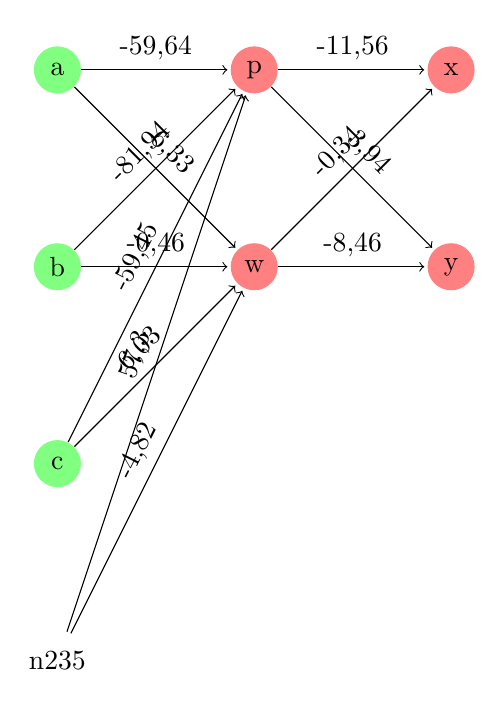
\begin{tikzpicture}[shorten >=1pt,->,draw=black!,node distance=2.5cm]
\tikzstyle{neuron}=[circle,fill=black!25,minimum size=17pt,inner sep=0pt]
\tikzstyle{constant}=[neuron, fill=white!50];
\tikzstyle{sigmoid}=[neuron, fill=red!50];
\tikzstyle{identity}=[neuron, fill=green!50];
\node [identity] (a) {a};
\node [identity,below of=a] (b) {b};
\node [identity,below of=b] (c) {c};
\node [constant,below of=c] (n235) {n235};
\node [sigmoid,right of=a] (p) {p};
\node [sigmoid,below of=p] (w) {w};
\node [sigmoid,right of=p] (x) {x};
\node [sigmoid,below of=x] (y) {y};
\path[every node/.style={sloped,anchor=south,auto=false}]
(w) edge node {-8,46} (y)
(w) edge node {-0,34} (x)
(p) edge node {-11,56} (x)
(p) edge node {3,94} (y)
(n235) edge node {-4,82} (w)
(n235) edge node {57,3} (p)
(c) edge node {6,03} (w)
(c) edge node {-59,45} (p)
(b) edge node {-0,46} (w)
(b) edge node {-81,94} (p)
(a) edge node {-59,64} (p)
(a) edge node {6,33} (w)
;\end{tikzpicture}
\end{document}